%\documentclass[compress,t,11pt]{beamer}
\documentclass[handout,compress,t,11pt]{beamer}
\usetheme[]{metropolis}           % Use metropolis theme
\usefonttheme{serif}
\definecolor[named]{Gray}{RGB}{111,112,114}
\definecolor[named]{DarkGray}{RGB}{48,48,48}
\definecolor[named]{Cardinal}{RGB}{179,22,34}
\usepackage[T1]{fontenc}
\usepackage[altbullet]{lucidabr}
\usepackage{textcomp}
\usepackage{upquote} % needed to make straight quotes work in listings
\usepackage{listgolang}
\usepackage{mathtools}
\usepackage{comment}
\usepackage{tikz}
\usepackage{tikzsymbols}
 \usetikzlibrary{trees,shapes,plotmarks,arrows,er,automata,petri,topaths,positioning}
\usepackage{pifont}
\usepackage{clrscode}
\usepackage{setspace}
\usepackage{soul}
\usepackage{hyperref}

\setbeamercolor{palette primary}{fg=white,bg=Cardinal}
\setbeamercolor{palette secondary}{fg=white,bg=Gray}
\setbeamercolor{palette tertiary}{fg=white,bg=Cardinal}
\setbeamercolor{palette quaternary}{fg=white,bg=Gray}
\setbeamercolor{palette sidebar primary}{fg=white,bg=Cardinal}
\setbeamercolor{palette sidebar secondary}{fg=white,bg=Gray}
\setbeamercolor*{titlelike}{fg=Cardinal}
\setbeamercolor{structure}{fg=Gray}
\setbeamercolor{title separator}{fg=Cardinal}
\setbeamercolor{alerted text}{fg=Cardinal}
\setbeamercolor{reversed}{fg=Cardinal,bg=black}

\newcommand{\card}[1]{\ensuremath{\left|#1\right|}}
\newcommand{\norm}[1]{\ensuremath{\|#1\|}}

\title[Programming in Go]{\bf Programming in Go\\ Lesson 4: Objects, Methods \& Interfaces}
\author{Matt Holiday} 
\institute[CP]{Cardinal Peak}
\date{7 May 2019} 
%\titlegraphic{\hfill
\includegraphics[width=.25\textwidth,height=.25\textheight]{cp-logo-2x.png}}
\titlegraphic{
\begin{tikzpicture}[overlay, remember picture,scale=0.4]
\node[at=(current page.north east), anchor=north east] (a) {};
\node[below left = 0.1cm and 0.1cm of a] (b)
{
\includegraphics[width=.25\textwidth,height=.25\textheight]{cp-logo-2x.png}};
\node[below left=2.4cm and 2.9cm of b]
{
\includegraphics[width=.2\textwidth]{go-may-fourth.jpg}};
\end{tikzpicture}}

\setbeamerfont{footline}{series=\bfseries\selectfont}
\setbeamersize{text margin left=12pt,text margin right=12pt}
\linespread{1.0}
\metroset{block=fill}

\hypersetup{
    colorlinks=true,
    linkcolor=Cardinal,
    filecolor=magenta,      
    urlcolor=blue,
}

\begin{document}
\frame{\titlepage} 

%\section{Introduction}
\begin{frame}[fragile]
    \frametitle{Lesson \#4}
    What we'll cover today:
    \begin{itemize}
    \item Homework \#3
    \item Object-oriented programming in Go
    \item Binding methods to objects
    \item Composing with \verb|struct|
    \item Interfaces
    \item Nil and empty interfaces
    \item Sorting
    \end{itemize}
\end{frame}


% =================================================================================

\begin{frame}[fragile]
    \frametitle{Homework \#3}
    Sample output: 2144 comics as of 5/4/2019 \par
{\small
\begin{verbatim}
$ go run main.go --get xkcd.json
skipping 404: got 404
skipping 2146: got a 404
skipping 2147: got a 404
. . .
skipping 2198: got a 404
skipping 2199: got a 404
read 2144 comics

$ go run main.go --find "Someone is in bed" xkcd.json
read 2144 comics
https://xkcd.com/571/ 4/20/2009
found 1 comics
\end{verbatim}}
\end{frame}

\begin{frame}[fragile]
    \frametitle{Homework \#3}
\begin{golang}
package main

import (
	"encoding/json"
	"flag"
	"fmt"
	"io"
	"net/http"
	"os"
	"strings"
)
\end{golang}
\end{frame}

\begin{frame}[fragile]
    \frametitle{Homework \#3}
\begin{golang}
// { "month":      "4",
//   "num":        571,
//   "year":       "2009",
//   . . .
//   "transcript": "[[Someone is in bed, . . . long int.",
//   "img":        "https://imgs.xkcd.com/comics/cant_sleep.png",
//   "title":      "Can't Sleep",
//   "day":        "20"
// }

type xkcd struct {
	Num        int    `json:"num"`
    Day        string `json:"day"`
    Month      string `json:"month"`
	Year       string `json:"year"`
	Title      string `json:"title"`
	Transcript string `json:"transcript"`
}
\end{golang}
\end{frame}

\begin{frame}[fragile]
    \frametitle{Homework \#3}
\begin{golang}
func getOne(i int) []byte {
    url := fmt.Sprintf("https://xkcd.com/%d/info.0.json", i)
	resp, err := http.Get(url)

	if err != nil {
		fmt.Fprintf(os.Stderr, "stopped reading: %s\n", err)
		os.Exit(-1)
	}

	defer resp.Body.Close()
\end{golang}
\end{frame}

\begin{frame}[fragile]
    \frametitle{Homework \#3}
\begin{golang}
	if resp.StatusCode != http.StatusOK {
		// easter egg: #404 returns HTTP 404 - not found

		fmt.Fprintf(os.Stderr, "skipping %d: got %d\n", 
                    i, resp.StatusCode)
		return nil
	}

	body, err := ioutil.ReadAll(resp.Body)

	if err != nil {
		fmt.Fprintf(os.Stderr, "bad body: %s\n", err)
		os.Exit(-1)
	}

	return body
}
\end{golang}
\end{frame}

\begin{frame}[fragile]
    \frametitle{Homework \#3}
\begin{golang}
var (
    getFlag  = flag.Bool("get", false, "fetch items")
    termFlag = flag.String("find", "", "term to search for")
)

func main() {
	flag.Parse()

	if *getFlag {
		// we're going to get all the entries and write
		// them one at a time to the output file (or stdout)

		var (
			output io.WriteCloser = os.Stdout
			err    error
			cnt    int
            data   []byte
		)
\end{golang}
\end{frame}

\begin{frame}[fragile]
    \frametitle{Homework \#3}
\begin{golang}
    	if len(flag.Args()) > 0 {
    		output, err = os.Create(flag.Arg(0))

    		if err != nil {
    			fmt.Fprintf(os.Stderr, "bad file: %s", err)
    			os.Exit(-1)
    		}

    		defer output.Close()
    	}

    	// the output will be in the form of a JSON array,
    	// so add the brackets before and after

    	fmt.Fprint(output, "[")
    	defer fmt.Fprint(output, "]")
\end{golang}
\end{frame}

\begin{frame}[fragile]
    \frametitle{Homework \#3}
\begin{golang}
        for i := 1; i < 2200; i++ {
            if data = getOne(i); data == nil {
                continue
            }

			if cnt > 0 {
				fmt.Fprint(output, ",")  // OB1
			}

			_, err = io.Copy(output, bytes.NewBuffer(data))

            if err != nil {
				fmt.Fprintf(os.Stderr, "stopped: %s", err)
				os.Exit(-1)
			}

            cnt++
		}
\end{golang}
\end{frame}

\begin{frame}[fragile]
    \frametitle{Homework \#3}
\begin{golang}
		fmt.Fprintf(os.Stderr, "read %d comics\n", cnt)
		return
	}

    // if we get here we are doing the "find" function
    // let's make sure we've got valid command-line inputs

	if len(*termFlag) == 0 {
		fmt.Fprintln(os.Stderr, "no search term")
		os.Exit(-1)
	}

	if len(flag.Args()) < 1 {
		fmt.Fprintln(os.Stderr, "no file given")
		os.Exit(-1)
	}
\end{golang}
\end{frame}

\begin{frame}[fragile]
    \frametitle{Homework \#3}
\begin{golang}
	var (
        items []xkcd
	    input io.ReadCloser
	    cnt   int
        err   error
    )

	if input, err = os.Open(flag.Arg(0)); err != nil {
		fmt.Fprintf(os.Stderr, "invalid file: %s", err)
		os.Exit(-1)
	}

	if err = json.NewDecoder(input).Decode(&items); err != nil {
		fmt.Fprintf(os.Stderr, "decode failed: %s\n", err)
		os.Exit(-1)
	}

	fmt.Fprintf(os.Stderr, "read %d comics\n", len(items))
\end{golang}
\end{frame}

\begin{frame}[fragile]
    \frametitle{Homework \#3}
\begin{golang}
	for _, v := range items {
		if strings.Contains(v.Title, *termFlag) || 
           strings.Contains(v.Transcript, *termFlag) {
			fmt.Printf("https://xkcd.com/%d/ %s/%s/%s\n", 
                       v.Num, v.Month, v.Day, v.Year)
			cnt++
		}
	}

	fmt.Fprintf(os.Stderr, "found %d comics\n", cnt)
}
\end{golang}
\end{frame}

% =================================================================================

% What's the point of object-oriented programming?
%
% The only way to handle complexity is to break it down into pieces, and if
% possible, hide most of it inside those pieces
%
% We need to limit the ways in which parts of the program can interact
%
% The basic idea is often expressed as ``separation of concerns''
% We separate the DB part from the logic part from the user interface part
% 
% OO modelling is an extension; wrap up pieces of state into an object with
% methods to provide limited behavior
%
% Abstraction - simplify the interface to a complex piece of the system
% Encapsulation - we have to hide stuff or the abstraction breaks down
%
% We use interfaces to get abstraction, and methods to provide the actual
% behavior to fulfill the abstraction
%
% Inheritance is one way to get dynamic execution; interfaces are another
% way that's actually a bit simpler
%
% And we can use structure embedding to get the sharing that inheritance
% is sometimes used for, without some of the complexity
%
% Inheritance has been overused; deep hierarchies have been a bomb; OO
% programming can turn into complex, bloated s/w if misused (Java shows this)



\section{Object-Oriented Programming}
\begin{frame}[fragile]
    \frametitle{What does that mean?}
    For many people, the essential elements of object-oriented programming
    have been:
    \begin{itemize}
        \item abstraction
        \item encapsulation
        \item polymorphism
        \item inheritance
    \end{itemize}
    \vspace{0.4\baselineskip}
    Sometimes those last two items are combined or confused \par
    \vspace{3\baselineskip}
    Go's approach to OO programming is similar but different
\end{frame}

\begin{frame}[fragile]
    \frametitle{Abstraction}
    Abstraction: decoupling behavior from the implementation details \par
    \vspace{\baselineskip}
    The Unix file system API is a great example of effective abstraction \par
    \vspace{0.4\baselineskip}
    Roughly five basic functions hide all the messy details:
    \begin{itemize}
        \item open
        \item close
        \item read
        \item write
        \item ioctl
    \end{itemize}
    \vspace{\baselineskip}
    Many different operating system things can be treated like files
\end{frame}

\begin{frame}[fragile]
    \frametitle{Encapsulation}
    Encapsulation: hiding implementation details from misuse \par
    \vspace{\baselineskip}
    It's hard to maintain an abstraction if the details are exposed: \par
    \begin{itemize}
        \item the internals may be manipulated in ways contrary to 
              the concept behind the abstraction
        \item users of the abstraction may come to depend on the
              internal details --- but those might change
    \end{itemize}
    \vspace{0.6\baselineskip}
    Encapsulation usually means controlling the visibility of names \\
    (``private'' variables) \par
\end{frame}

\begin{frame}[fragile]
    \frametitle{Polymorphism}
    Polymorphism literally means ``many shapes'' --- multiple types behind
    a single interface \par
    \vspace{0.4\baselineskip}
    Three main types are recognized:
    \begin{itemize}
        \item ad-hoc: typically found in function/operator overloading
        \item parametric: this is what generic programming is about
        \item subtype: subclasses substituting for superclasses
    \end{itemize}
    \vspace{\baselineskip}
    ``Protocol-oriented'' programming uses explicit interface types,\\
    now supported in many popular languages (an ad-hoc method) \par
    \vspace{\baselineskip}
    In this case, behavior is completely separate from implementation,\\
    which is good for abstraction
\end{frame}

\begin{frame}[fragile]
    \frametitle{Inheritance}
    Inheritance has conflicting meanings:
    \begin{itemize}
        \item substitution (subtype) polymorphism
        \item structural sharing of implementation details
    \end{itemize}
    \vspace{\baselineskip}
    In theory, inheritance should always imply subtyping: \\the subclass should
    be a ``kind of'' the superclass \par
    \vspace{\baselineskip}
    See the \href{https://en.wikipedia.org/wiki/Liskov_substitution_principle}%
    {Liskov substitution principle} \par
    \vspace{\baselineskip}
    Theories about substitution can be pretty messy
\end{frame}

\begin{frame}[fragile]
    \frametitle{Why would inheritance be bad?}
    Inheritance injects a dependence on the superclass into the subclass:
    \begin{itemize}
        \item what if the superclass changes behavior?
        \item what if the subclass never really met the abstract concept?
    \end{itemize}
    \vspace{\baselineskip}
    Deep inheritance hierarchies have proven to be fragile \par
    \vspace{\baselineskip}
    Not having inheritance means better encapsulation \& isolation \par
    \vspace{1.6\baselineskip}
    ``Interfaces will force you to think in term of communication between objects'' --- Nicolò Pignatelli
    in \href{https://codeburst.io/inheritance-is-evil-stop-using-it-6c4f1caf5117}{Inheritance is evil} \par
    \vspace{0.4\baselineskip}
    See also \href{https://en.wikipedia.org/wiki/Composition_over_inheritance}%
    {Composition over inheritance}
\end{frame}

\begin{frame}[fragile]
    \frametitle{OO in Go}
    Go offers four main supports for OO programming:
    \begin{itemize}
        \item encapsulation using the package for visibility control
        \item abstraction \& polymorphism using interface types
        \item enhanced {\em composition} to provide structure sharing
    \end{itemize}
    \vspace{\baselineskip}
    Go does not offer inheritance or substitutability based on types \par
    \vspace{\baselineskip}
    Substitutability is based only on {\bf interfaces}: purely a function of 
    abstract {\bf behavior} \par
    \vspace{2\baselineskip}
    See \href{http://talks.golang.org/2014/go4gophers.slide#1}{Go for Gophers}
\end{frame}

% =================================================================================

\section{Methods}
\begin{frame}[fragile]
    \frametitle{Methods are type-bound functions}
    A ``method'' is a special type of function with a special syntax \par
    \vspace{0.4\baselineskip}
    It has a ``receiver'' parameter and uses ``dot'' notation in calls
\begin{golang}
type Pair struct {
    Path string
    Hash string
}

func (p Pair) String() string {
    return fmt.Sprintf("Hash of %v is %v", p.Path, p.Hash)
}

s := p.String()
\end{golang}
    \vspace{0.4\baselineskip}
    And so it's grouped into the ``method set'' of a type
\end{frame}

\begin{frame}[fragile]
    \frametitle{So why have methods?}
    This is not just about notation: calling \verb|x.Do()| \par
    \vspace{0.4\baselineskip}
    Only methods may be used to satisfy an {\em interface}
    \vspace{\baselineskip}
\begin{golang}
type Stringer interface {
    func String() string
}

func (p Pair) String() string {
    return fmt.Sprintf("Hash of %v is %v", p.Path, p.Hash)
}

var s Stringer = p
\end{golang}
    \vspace{\baselineskip}
    Methods can't be closures because that would be too complex
\end{frame}

\begin{frame}[fragile]
    \frametitle{Not just structs}
    A method may be defined on any {\bf named} type \par
    \vspace{0.4\baselineskip}
    That means methods can't be declared on \verb|string|, but
    \vspace{\baselineskip}
\begin{golang}
type StringSlice []string

func (s StringSlice) String() string {
    // format and print the slice
}
\end{golang}
    \vspace{\baselineskip}
    The same method name may be bound to different types \par
    \vspace{\baselineskip}
    The package name is not required to qualify the method name
\end{frame}

\begin{frame}[fragile]
    \frametitle{Make the nil value useful}
\begin{golang}
package collection


type StringStack struct {
    data []string     // "zero" value ready-to-use
}


func (s *StringStack) Push(x string) {
    s.data = append(s.data, x)
}

func (s *StringStack) Size() int {
    return len(s.data)
}
\end{golang}
\end{frame}

\begin{frame}[fragile]
    \frametitle{Nil as a receiver value}
    Make \verb|nil| useful: handle it as a receiver when possible \par
    \vspace{0.4\baselineskip}
    Nothing in Go prevents calling a method with a nil receiver
    \vspace{\baselineskip}
\begin{golang}
// Sum returns the sum of the list elements.
func (list *IntList) Sum() int {
    if list == nil {
        return 0
    }

    return list.Value + list.Tail.Sum()
}
\end{golang}
\end{frame}


% ========================================================================================

\section{Composition, not Inheritance}
\begin{frame}[fragile]
    \frametitle{Composition}
    Go allows a new kind of composition (besides a normal field) \par
    \vspace{0.4\baselineskip}
    An embedded \verb|struct| appears to have its fields live at the
    same ``level'' as the structure it becomes a part of {\em (promotion)} \par
    \vspace{0.6\baselineskip}
\begin{golang}
type Pair struct {
    Path string
    Hash string
}

type PairWithLength struct {
    Pair
    Length int
}

pl := PairWithLength{Pair{"/usr", "0xfdfe"}, 121}
fmt.Println(pl.Path, pl.Length)  // not pl.x.Path
\end{golang}
\end{frame}

\begin{frame}[fragile]
    \frametitle{Composition}
    The {\em methods} of an embedded \verb|struct| are also promoted \par
    \vspace{\baselineskip}
    Those methods {\bf can't} see fields of the {\em embedding} \verb|struct|  \par
    \vspace{\baselineskip}
\begin{golang}
func (p Pair) String() string {
    return fmt.Sprintf("Hash of %v is %v", p.Path, p.Hash)
}

pl := PairWithLength{Pair{"/usr", "0xfdfe"}, 121}

// Pair.String() doesn't have visibility to pl.Length

fmt.Println(pl)   // prints "Hash of /usr is 0xfdfe"
\end{golang}
\end{frame}

\begin{frame}[fragile]
    \frametitle{Composition}
    The {\em methods} of an embedded \verb|struct| are also promoted \par
    \vspace{\baselineskip}
    Unless the new \verb|struct| later defines the same method on itself \par
    \vspace{\baselineskip}
\begin{golang}
pl := PairWithLength{Pair{"/usr", "0xfdfe"}, 121}

fmt.Println(pl) // uses Pair.String()

// now, if we later define the same method

func (p PairWithLength) String() string {
    return fmt.Sprintf("Length of %v is %v with hash %v", 
                       p.Path, p.Length, p.Hash)
}

fmt.Println(pl) // would now use PairWithLength.String
\end{golang}
\end{frame}

\begin{frame}[fragile]
    \frametitle{Composition is not inheritance}
    A \verb|PairWithLength| {\bf can't} substitute for a \verb|Pair| \par
    \vspace{\baselineskip}
    They are different and essentially unrelated types \par
    \vspace{\baselineskip}
\begin{golang}
func Filename(p Pair) string {
    return filepath.Base(p.Path)
}

pl := PairWithLength{Pair{"/usr", "0xfdfe"}, 121}

a := Filename(pl) // NOT ALLOWED even though pl.Path exists
\end{golang}
    \vspace{2\baselineskip}
    The only substitution is through interface types!
\end{frame}

\begin{frame}[fragile]
    \frametitle{Composition with pointer types}
    A struct can embed a pointer to another type; promotion of its fields 
    and methods works the same way \par
\begin{golang}
type Fizgig struct {
    *PairWithLength
    Broken bool
}

fg := Fizgig{
    &PairWithLength{
        Pair{"/usr", "0xfdfe"}, 
        121,
    },
    false,
}

fmt.Println(fg)
// Length of /usr is 121 with hash 0xfdfe
\end{golang}
\end{frame}


% =================================================================================

\section{Interface Types}

\begin{frame}[fragile]
    \frametitle{Interfaces}
    An interface type is a collection (aggregation) of methods \par
    \vspace{\baselineskip}
    They define an abstraction through behavior, like {\em abstract classes}\\
    in other languages \par
    \vspace{0.4\baselineskip}
    Any type which defines both these methods satisfies the interface: \par
\begin{golang}
type ReadWriter interface {
    Read(p []byte) (n int, err error)
    Write(p []byte) (n int, err error)
}
\end{golang}
    \vspace{\baselineskip}
    This is known as {\em structural} typing (``duck'' typing) \par
    \vspace{0.4\baselineskip}
    No type will declare itself to implement \verb|ReadWriter| explicitly
\end{frame}

\begin{frame}[fragile]
    \frametitle{Interface variables}
    A variable of interface type can refer to any object that satisfies it \par
    \vspace{0.4\baselineskip}
\begin{golang}
func io.Copy(w Writer, r Reader) (int, error) {
    . . .
}

f1, err := os.Open("input.txt")
f2, err := os.Open("output.txt")

n, err := io.Copy(f2, f1)
\end{golang}
    \vspace{0.6\baselineskip}
    Here \verb|w| and \verb|r| are references ultimately to files \par
    \vspace{0.4\baselineskip}
    But it could be a \verb|File| and a \verb|bytes.Buffer| source;
    it wouldn't\\
     care --- all it needs is the specific behaviors (write \& read)
\end{frame}

\begin{frame}[fragile]
    \frametitle{Interfaces}
    Interfaces are the basis for {\em substitutability} in Go \par
    \vspace{0.4\baselineskip}
\begin{golang}
type ByteCounter int

func (b *ByteCounter) Write(p []byte) (int, error) {
    *b += ByteCounter(len(p)) // convert int to ByteCounter
    return len(p), nil
}

var c ByteCounter

f, _ := os.Open("input.txt")
n, _ := io.Copy(c, f)
\end{golang}
    \vspace{\baselineskip}
    Lots of types are \verb|Writers| and can be written/copied to; \\
    see also Francesc Campoy \href{https://www.youtube.com/watch?v=F4wUrj6pmSI}%
    {Understanding Go Interfaces}
\end{frame}


\begin{frame}[fragile]
    \frametitle{Interfaces}
    An HTTP handler function is an instance of an interface
\begin{golang}
type Handler interface {
	ServeHTTP(ResponseWriter, *Request)
}
    
type HandlerFunc func(ResponseWriter, *Request)

func (f HandlerFunc) ServeHTTP(w ResponseWriter, r *Request) {
    f(w, r)
}

// handler matches type HandlerFunc and so interface Handler
// so the HTTP framework can call ServeHTTP on it

func handler(w http.ResponseWriter, r *http.Request) {
    fmt.Fprintf(w, "Hello, world! from %s\n", r.URL.Path[1:])
}
\end{golang}
\end{frame}

\begin{frame}[fragile]
    \frametitle{Interfaces}
    Interfaces are just types \& values orthogonal to the rest of Go
\begin{golang}
type Handler interface {
	ServeHTTP(ResponseWriter, *Request)
}

type HandlerFunc func(ResponseWriter, *Request)

func (f HandlerFunc) ServeHTTP(w ResponseWriter, r *Request) {
    f(w, r)
}
\end{golang}
\vspace{\baselineskip}
    Interfaces separate data from behavior (classes conflate them) \par
\vspace{\baselineskip}
    They provide a model of genericity (but not quite parametric polymorphism)    
\end{frame}

\begin{frame}[fragile]
    \frametitle{Interfaces and substitution}
    All the methods must be present to satisfy the interface \par
\begin{golang}
var w io.Writer

w = os.Stdout           // OK: *os.File has Write method
w = new(bytes.Buffer)   // OK: *bytes.Buffer has Write method
w = time.Second         // ERROR: no Write method

var rwc io.ReadWriteCloser

rwc = os.Stdout         // OK: *os.File has all 3 methods
rwc = new(bytes.Buffer) // ERROR: no Close method

w = rwc                 // OK: io.ReadWriteCloser has Write
rwc = w                 // ERROR: no Close method
\end{golang}
\end{frame}

\begin{frame}[fragile]
    \frametitle{Interface satisfiability}
    And the must be of the right type (pointer or value) \par
\begin{golang}
type IntSet struct { /* ... */ }

func (*IntSet) String() string

var _ = IntSet{}.String() // ERROR: String needs *IntSet

var s IntSet
var _ = s.String()        // OK: s is a variable and
                          // &s has String

var _ fmt.Stringer = &s   // OK
var _ fmt.Stringer = s    // ERROR: no String method
\end{golang}
\end{frame}

\begin{frame}[fragile]
    \frametitle{Interface also offer composition}
    \verb|ReadWriter| is actually defined by Go as two interfaces \par
\begin{golang}
type Reader interface {
    Read(p []byte) (n int, err error)
}

type Writer interface {
    Write(p []byte) (n int, err error)
}

type ReadWriter interface {
    Reader
    Writer
}
\end{golang}
    \vspace{\baselineskip}
    Small interfaces with composition where needed are more flexible \par
\end{frame}

\begin{frame}[fragile]
    \frametitle{Nil interfaces}
    An interface variable is \verb|nil| until initialized \par
    \vspace{0.4\baselineskip}
    It really has two parts:
    \begin{itemize}
        \item a value or pointer of some type
        \item a pointer to information about the type so
              the correct actual method can be identified
    \end{itemize}
\begin{golang}
var r io.Reader     // nil until initialized
var b bytes.Buffer  // ditto

r := b              // r is no longer nil!
                    // but it has a nil pointer to a Buffer
\end{golang}
    \vspace{0.2\baselineskip}
    This causes a lot of confusion! \par
    \vspace{0.2\baselineskip}
    An interface variable is \verb|nil| only if both parts are
\end{frame}

\begin{frame}[fragile]
    \frametitle{Nil interfaces}
    An interface variable is \verb|nil| until initialized \par
    \vspace{0.4\baselineskip}
    It really has two parts:
    \begin{itemize}
        \item a value or pointer of some type
        \item a pointer to information about the type so
              the correct actual method can be identified
    \end{itemize}
\begin{center}
    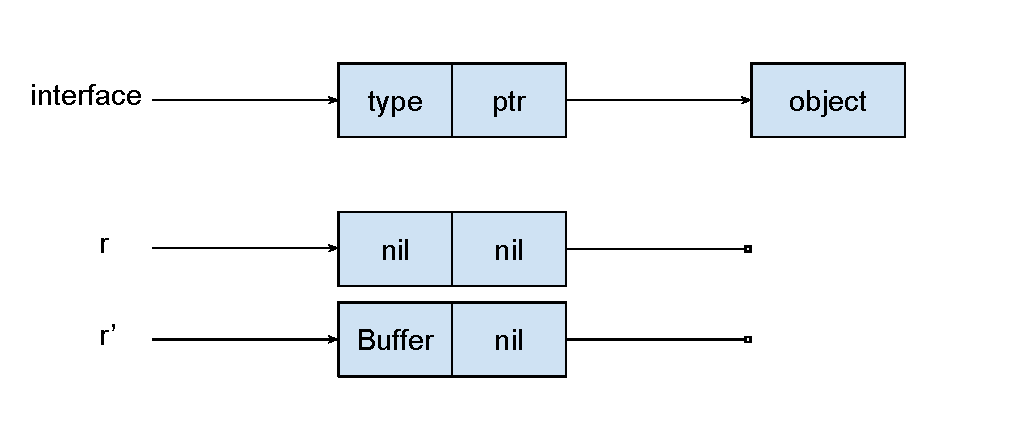
\includegraphics[width=0.9\textwidth]{interface-picture.pdf}
\end{center}
\end{frame}

\begin{frame}[fragile]
    \frametitle{Error is really an interface}
    We called \verb|error| a special type, but it's really an interface \par
\begin{golang}
type error interface {
    func Error() string
}
\end{golang}
    \vspace{0.6\baselineskip}
    We can compare it to \verb|nil| unless we make a mistake \par
\begin{golang}
var err error

func XYZ(a int) (int, *errFoo) {
    return 0, nil
}

n, err := XYZ(1)   // BAD: interface gets a nil concrete ptr
\end{golang}
\vspace{0.6\baselineskip}
See \href{https://golang.org/doc/faq#nil_error}{Why is my nil error value not equal to nil?}
\end{frame}

\begin{frame}[fragile]
    \frametitle{Empty interfaces}
    The \verb|interface{}| type has no methods \par
    \vspace{\baselineskip}
    So it is satisfied by anything! \par
    \vspace{\baselineskip}
    Empty interfaces are commonly used; they're how the formatted
    I/O routines can print any type
\begin{golang}
func fmt.Printf(f string, args ...interface{})
\end{golang}
    \vspace{2\baselineskip}
    {\em Reflection} is needed to determine what the concrete type is \par
    \vspace{0.4\baselineskip}
    We'll talk about that later
\end{frame}

% =================================================================================

\section{Sorting}

\begin{frame}[fragile]
    \frametitle{Sortable interface}
    \verb|sort.Interface| is defined as \par
\begin{golang}
type Interface interface {
    // Len is the number of elements in the collection.
    Len() int

    // Less reports whether the element with
    // index i should sort before the element with index j.
    Less(i, j int) bool

    // Swap swaps the elements with indexes i and j.
    Swap(i, j int)
}
\end{golang}
    \vspace{0.6\baselineskip}
    and \verb|sort.Sort| as \par
\begin{golang}
func Sort(data Interface)
\end{golang}
\end{frame}

\begin{frame}[fragile]
    \frametitle{Sortable built-ins}
    Slices of strings can be sorted using \verb|StringSlice| \par
    \vspace{\baselineskip}
\begin{golang}
//  defined in the sort package
//  type StringSlice []string

entries := []string{"charlie", "able", "dog", "baker"}

sort.Sort(sort.StringSlice(entries))

fmt.Println(entries)   // [able baker charlie dog]
\end{golang}
\end{frame}

\begin{frame}[fragile]
    \frametitle{Sorting example}
    Implement  \verb|sort.Interface| to make a type sortable: \par
    \vspace{\baselineskip}
\begin{golang}
type Organ struct {
    Name   string
    Weight int
}

type Organs []Organ

func (s Organs) Len() int      { return len(s) }
func (s Organs) Swap(i, j int) { s[i], s[j] = s[j], s[i] }
\end{golang}
\vspace{3\baselineskip}
From Andrew Gerrand's \href{https://talks.golang.org/2014/go4gophers.slide#1}{Go for gophers}
\end{frame}

\begin{frame}[fragile]
    \frametitle{Sorting example}
    Implement  \verb|sort.Interface| to make a type sortable: \par
    \vspace{0.6\baselineskip}
\begin{golang}
type ByName struct{ Organs }

func (s ByName) Less(i, j int) bool { 
    return s.Organs[i].Name < s.Organs[j].Name 
}

type ByWeight struct{ Organs }

func (s ByWeight) Less(i, j int) bool { 
    return s.Organs[i].Weight < s.Organs[j].Weight
}
\end{golang}
    \vspace{0.6\baselineskip}
    Here we use {\em struct composition} which promotes the \verb|Organs| methods
\end{frame}

\begin{frame}[fragile]
    \frametitle{Sorting example}
    Make a struct of the correct type on the fly to sort: \par
\begin{golang}
    s := []Organ{
        {"brain", 1340},
        {"heart", 290},
        {"liver", 1494},
        {"pancreas", 131},
        {"spleen", 162},
    }

    sort.Sort(ByWeight{s})      // pancreas first
    fmt.Println(s)

    sort.Sort(ByName{s})        // brain first
    fmt.Println(s)
\end{golang}
{\scriptsize
\begin{verbatim}
[{pancreas 131} {spleen 162} {heart 290} {brain 1340} {liver 1494}]
[{brain 1340} {heart 290} {liver 1494} {pancreas 131} {spleen 162}]
\end{verbatim}}
\end{frame}

\begin{frame}[fragile]
    \frametitle{Sorting in reverse}
    Use \verb|sort.Reverse| which is defined as: \par
\begin{golang}
type reverse struct {
	// This embedded Interface permits Reverse to use the 
    // methods of another Interface implementation.
	Interface
}

// Less returns the opposite of the embedded implementation's 
// Less method.
func (r reverse) Less(i, j int) bool {
	return r.Interface.Less(j, i)
}

// Reverse returns the reverse order for data.
func Reverse(data Interface) Interface {
	return &reverse{data}
}
\end{golang}
\end{frame}

\begin{frame}[fragile]
    \frametitle{Sorting in reverse}
    Let's use \verb|StringSlice| again: \par
    \vspace{\baselineskip}
\begin{golang}
//  defined in the sort package
//  type StringSlice []string

entries := []string{"charlie", "able", "dog", "baker"}

sort.Sort(sort.Reverse(sort.StringSlice(entries)))

fmt.Println(entries)   // [dog charlie baker able]
\end{golang}
\end{frame}

% =================================================================================

\section{Details, Details}
\begin{frame}[fragile]
    \frametitle{Pointer vs value receivers}
    A method can be defined on a pointer to a type \par
    \vspace{0.4\baselineskip}
    In this case, the receiver is passed ``by reference''
\begin{golang}
type Point struct {
	x,y float32
}

func (p *Point) Add(x, y float32) {
	p.x, p.y = p.x + x, p.y + y
}

func (p Point) OffsetOf(p1 Point) (x float32, y float32) {
	x, y = p.x - p1.x, p.y - p1.y
	return
}
\end{golang}
The same method name may {\bf not} be bound to both \verb|T| and \verb|*T| \par
\end{frame}

\begin{frame}[fragile]
    \frametitle{Pointer vs value receivers}
    Pointer methods may be called on non-pointers and vice versa \par
    \vspace{\baselineskip}
    Go will automatically use \verb|*| or \verb|&| as needed \par
\begin{golang}
p1 := new(Point)     // *Point, at (0,0)
p2 := Point{1, 1}

p1.OffsetOf(p2)      // same as (*p1).OffsetOf(p2)

p2.Add(3, 4)         // same as (&p2).Add(3, 4)
\end{golang}
\vspace{2\baselineskip}
Except \verb|&| may only be applied to objects that are {\em addressable}
\end{frame}

\begin{frame}[fragile]
    \frametitle{Pointer vs value receivers}
    Compatibility between objects and receiver types \par
\begin{center}
\begin{table}[h!]
{\renewcommand{\arraystretch}{1.7}%
    \begin{tabular}{l|l|l|l}
    & \textbf{Pointer} & \textbf{L-Value} & \textbf{R-Value} \\
    \hline
    pointer receiver & OK & OK \verb|&| & \alert{\bf Not OK}  \\
    \hline
    value receiver & OK \verb|*| & OK & OK
    \end{tabular}}
\end{table}
\end{center}
A method requiring a pointer receiver may only be called on an addressable object
\begin{golang}
var p Point

p.Add(1, 2)               // OK, &p
Point{1, 1}.Add(2, 3)     // Not OK, can't take address
\end{golang}
\end{frame}

\begin{frame}[fragile]
    \frametitle{Consistency in receiver types}
    If a type has a method with a pointer receiver, then all its methods
    should take pointers \par
    \vspace{0.4\baselineskip}
    And in general objects of that type are probably not safe to copy
\begin{golang}
type Buffer struct {
	buf       []byte
	off       int
    . . .
}

func (b *Buffer) ReadString(delim byte) (string, error) {
	. . .
}
\end{golang}
Copying a \verb|Buffer| object will cause both copies to reference the same
underlying byte slice --- bad news in most cases
\end{frame}

\begin{frame}[fragile]
    \frametitle{Method values}
    A selected method may be passed similar to a closure; the receiver is closed 
    over at that point
    \vspace{0.4\baselineskip}
\begin{golang}
func (p Point) Distance(q Point) float64 {
    return math.Hypot(q.X-p.X, q.Y-p.Y)
}

p := Point{1, 2}
q := Point{4, 6}

distanceFromP := p.Distance    // this is a method value

fmt.Println(distanceFromP(q))  // and can be called later
\end{golang}
    \vspace{0.4\baselineskip}
The value of \verb|p| is copied into the method value because \verb|Distance| takes 
a {\em value} receiver; if \verb|p| took a pointer receiver, it would have a reference 
to \verb|p| and calculate based on \verb|p|'s most current value
\end{frame}


% =================================================================================

\section{Homework}

\begin{frame}[fragile]
\frametitle{Homework \#4}
Exercise 7.11 from {\em GOPL:} web front-end for a database \par
    \vspace{0.4\baselineskip}
{\small \setstretch{1.1}Add additional handlers [to the database example in \S7.7,
which is program \verb|gopl.io/ch7/http4|]
so that clients can create, read, update, and delete database entries. For example, 
a request of the form 
\begin{verbatim}
    /update?item=socks&price=6
\end{verbatim}
will update the price of an item in the inventory and report an error if \\
the item does not exist or if the price is invalid. \par
    \vspace{0.4\baselineskip}
(Warning: this change introduces concurrent 
variable updates --- but we will {\em ignore} the race conditions for the purpose
of this exercise.) \par
    \vspace{0.4\baselineskip}
(Note: I dropped the \verb|price| method from my solution, since it overlaps the
new \verb|read| operation.)}
\end{frame}

\end{document}
